\documentclass[twocolumn,letterpaper]{article}

\usepackage{times}
\usepackage[protrusion=true,expansion=true]{microtype} % Better typography
\usepackage[T1]{fontenc}

\usepackage[margin=1.0in,includefoot]{geometry}

\usepackage{titlesec}
\titleformat*{\section}{\bfseries\sffamily\large}
\titleformat*{\subsection}{\bfseries\sffamily\normalsize}

\usepackage{natbib}
\usepackage{graphicx}

\usepackage{lipsum}

\title{The Answers to Important Questions}
\author{Jane Smith, Ph.D.}
\date{\today}

\begin{document}

\twocolumn[
  \begin{@twocolumnfalse}
    \maketitle

    {\bfseries\sffamily\normalsize Abstract}\vspace{1ex}

    Lorem ipsum dolor sit amet, consectetuer adipiscing elit. Ut purus
    elit, vestibulum ut, placerat ac, adipiscing vitae,
    felis. Curabitur dictum gravida mauris. Nam arcu libero, nonummy
    eget, consectetuer id, vulputate a, magna. Donec vehicula augue eu
    neque. Pellentesque habitant morbi tristique senectus et netus et
    malesuada fames ac turpis egestas. Mauris ut leo. Cras viverra
    metus rhoncus sem. Nulla et lectus vestibulum urna fringilla
    ultrices. Phasellus eu tellus sit amet tortor gravida
    placerat. Integer sapien est, iaculis in, pretium quis, viverra
    ac, nunc. Praesent eget sem vel leo ultrices bibendum. Aenean
    faucibus. Morbi dolor nulla, malesuada eu, pulvinar at, mollis ac,
    nulla. Curabitur auctor semper nulla. Donec varius orci eget
    risus. Duis nibh mi, congue eu, accumsan eleifend, sagittis quis,
    diam. Duis eget orci sit.

    \vspace{6ex}
  \end{@twocolumnfalse}
]

\section*{Introduction}

\lipsum[1]

Here is a reference to an article \citep{hodgkin1952propagation}.

\lipsum[1-4]

\section*{Methods}

\subsection*{Subjects}

\lipsum[1]

\subsection*{Procedures}

\lipsum[1-5]

\subsection*{Statistical Analyses}

Equation~\ref{eq:mean} shows the equation for calculating the mean of
$N$ values $X_{1}$ to $X_{N}$.

\begin{equation}
  \bar{X} = \left( \frac{1}{N}  \right) \sum_{i=1}^{N} X_{i}
  \label{eq:mean}
\end{equation}


\lipsum[1]

\section*{Results}

As you can see in Figure~\ref{fig:subjectmeans}, we have collected
some data already.

\begin{figure}
  \centering
  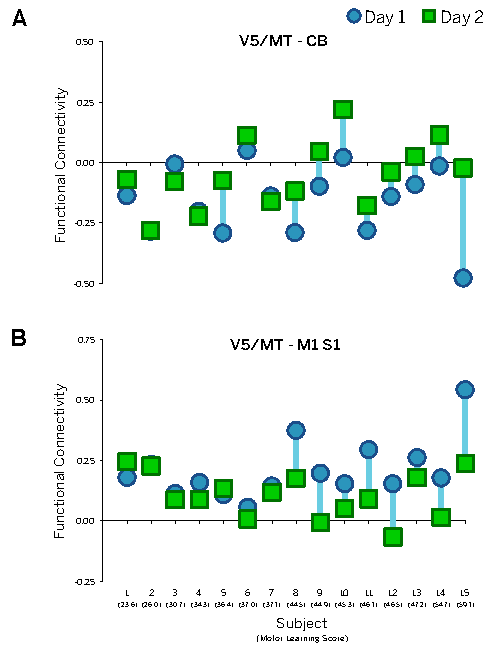
\includegraphics[width=\columnwidth]{figure.pdf}
  \caption{Some data from our experiment.}
  \label{fig:subjectmeans}
\end{figure}    

\lipsum[1-2]

Table~\ref{tab:randomjunk} shows some data organized into a table.

\begin{table}
  \centering
  \begin{tabular}{|r|l|}
    \hline
    \textbf{Value} & \textbf{Format}\\
    \hline\hline
  7C0 & hexadecimal \\
  3700 & octal \\ \cline{2-2}
  11111000000 & binary \\
  \hline
  1984 & decimal \\
  \hline
  \end{tabular}
  \caption{Some data.}
  \label{tab:randomjunk}
\end{table}

\lipsum[1-2]

\section*{Discussion}

\lipsum[1-10]

\bibliography{refs}
\bibliographystyle{jneurosci}

\end{document}



